%:
\documentclass[11pt, oneside]{article}   	% use "amsart" instead of "article" for AMSLaTeX format
\usepackage{geometry}                		% See geometry.pdf to learn the layout options. There are lots.
\geometry{letterpaper}                   		% ... or a4paper or a5paper or ... 
%\geometry{landscape}                		% Activate for rotated page geometry
%\usepackage[parfill]{parskip}    		% Activate to begin paragraphs with an empty line rather than an indent
\usepackage{graphicx}				% Use pdf, png, jpg, or eps§ with pdflatex; use eps in DVI mode
								% TeX will automatically convert eps --> pdf in pdflatex		
\usepackage{amssymb}
\usepackage{diagbox}
\usepackage{amsmath}
\usepackage{amsthm}
\usepackage{enumerate}
\usepackage{tikz}
\usepackage{mathrsfs}
\usetikzlibrary{positioning}


\usetikzlibrary{arrows}
\theoremstyle{definition}
\newtheorem*{defn}{Definition}
\newtheorem*{prop}{Proposition}
\newtheorem*{eg}{Example}
\newtheorem*{thm}{Theorem}
\newtheorem*{corol}{Corollary}
\newtheorem{ex}{Exercise}[section]
{\theoremstyle{plain}
\newtheorem*{rmk}{Remark}
\newtheorem*{rmks}{Remarks}
\newtheorem*{lt}{Last time}
}
\newtheorem*{lem}{Lemma}
\usepackage{color}
\usepackage{CJK}
\title{Path to Efficient AGI}
\author{Xiyu Zhai}
\date{}							% Activate to display a given date or no date

\begin{document}
\maketitle
\tableofcontents


\section{Introduction}

(Warning: draft in progress. This is not meant for publication at a specific conference, but a central bus where different ideas are organised and described in a coherent way.)

This paper discusses the optimal path to sample and computation efficient AGI in the era of deep learning. We first confirm theoretically the capabilities of deep learning as general purpose end-to-end machine learning methods, then argue a school of domain specific modular machine learning methods powered by a new programming language will replace deep learning as the best path to AGI.

To give insights, we make some high level discussions.

\paragraph {General Purpose vs Domain Specific.} In many fields, general purpose methods are worse than highly optimized domain specific ones. For example,
\begin{itemize}
	\item Matlab, Mathematica are domain specific programming languages, more effective to use than C++/python for many specific circumstances;
	\item for specific computation tasks, specfically designed data structures are better than general purpose ones, like `SmallVec' rather than `Vec'
	\item in mathematics, PDE domain specific techniques are more powerful than general purpose functional analysis tools.
\end{itemize}

However, in the field of AI, general purpose methods seem to perform better. People no longer use domain specific feature engineering as a decade ago. Everything is some kind of neural network.

We believe the apparent worse performance of domain specific AI techniques is largely due to engineering challenges. On one hand, feature engineering and rule based system historically failed due to either shortage of engineering efforts or inability to exploit specific domain. On the other hand, deep learning can scale easily with more data and computation are advanced by the joint effort of countless researchers and engineers around the globe.

\paragraph {End-to-End vs Modular} By definition, "modular" is a better property in terms of debuggability, robustness, flexibility. However, under the current deep-learning based AI frameworks, modularity is harder to achieve than end-to-end.

\paragraph {New Programming Language Design}
We propose a new programming language design that would make AI engineering much more efficient, allowing domain specific models that perform much better than general purpose end-to-end methods.

The language shall address challenges in the three major aspects:

\begin{itemize}
	\item Inference. The domain specifically optimal inference could involve computation other than matrix algebra, the language shall be able to \textbf{implement quickly system level algorithms} that are the building blocks of the overall model; furthermore, queries could be repetitive with each other in some aspects, so the language shall be able to support \textbf{incremental computation and memoization}. Lastly, we desire modular rather than end-to-end models, so the language shall support \textbf{distribute features across modules and packages}. 
	\item Training. Gradient descent cannot be used because the proper hypothesis class will not be smoothly parametrizable in general (say, each hypothesis is a rule database, or a Rust program). So the language shall allow us to \textbf{write sophisticated domain specific (symbolic) searching algorithms for training}. We may ease the optimization difficulty by labeling some intermediate features either manually or through pretrained deep learning models, so language need to \textbf{make it trivial to integrate with manual labeling or derived label functions}. It's also possible to adapt the training process, i.e. language need to support \textbf{higher order machine learning}.
	\item Development. In traditional programming, we largely have clear ideas about what we do beforehand and then write code to implement them; however, in domain specific AI engineering, we need to interact to know what to do. For example, we surmise that a certain feature based on a geometric function of curves will work for MNIST, only to find that it performs good overall except a few cases. We then need to narrow down to those cases and see what's happening. It might be our idea is wrong, or might be the code is buggy, or these cases are just not meant for this function. We need an \textbf{interactive, fully debuggable and visualizable IDE system that display inputs, labels, features for either the whole dataset, or a specific subset or just a single point}.
\end{itemize}

We shall give a more detailed explanation in section ??. But the full specification will be given in a separated paper.

If successful, we shall be able to invent domain specific AI techniques that 

\begin{itemize}
	\item Inference is more efficient, robust and explainable. Could have language models without illusion yet 1000 times faster, runnable on local device.
	\item Training.
	\item Development.
\end{itemize}
 In the date of writing, the language is close to a new working version, including more than 90k lines of Rust code.

\section{Related Works}

\section{Main Results}

\subsection{Neural Network Expressive Power}


\section{Modular Pattern Recognition Graph}

\begin{quote}
The greatest benefit to recognizing patterns is that it gives you a pathway to power, and a ladder out of chaos. \\
\emph{Tony Robbins}
\end{quote}


Here we introduce a framework to describe the computation process of pattern recognition.

\subsection{Pattern Recognition}

Intuitively pattern recognition is a function that is (using classical computers)
\begin{itemize}
	\item computable. For the very least, in polynomial time and space.
	\item learnable. Either theoretically or empirically.
\end{itemize}

The importance of computability is needless to say. Learnability is critical for scaling, because it's much cheaper to train on machines than hiring millions of programmers to hand write everything.

Examples of pattern recognitions are

\begin{itemize}
	\item Linear function. Computability is obviously. It's learnable both theoretically and empirically.
	\item Various tasks in computer vision. Empirically shown by neural networks.
	\item Various tasks in natural language processing. Empirically shown by neural networks.
\end{itemize}

Neural networks themselves are not viewed as "pattern recognition" because they can be hard to learn (the learning problem in neural networks is NP-complete, shown in Judd 1987, 1990).

\subsection{Computation Graph}


First, we use graph to represent a complicated function composed from simple ones. We use graph instead of DSL for the benefit of clarity.

This is not much different from those graphs for neural networks.

\begin{defn}[Computation Graph]
A computation graph is a directed graph with nodes being types, and for a node $T$, with a nonempty list of incoming edges, the starting node type of which are $S_1,\cdots,S_n$, there is a function $$f: (S_1,\cdots,S_n)\to T$$.
\end{defn}

All the nodes without incoming edges are seen as inputs, and all the nodes without outgoing edges are seen as outputs.

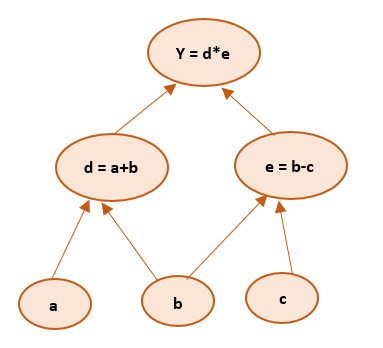
\includegraphics{computation_graph.png}

\subsection{Pattern Recognition Graph}

\subsection{Modular Pattern Recognition Graph}

Pattern recognition graph is a specialized computational graph such that it's computable, learnable, explainable and well-suited to a specific domain.

(Explainability is possible because we only allow nodes to be associated with explainably types, i.e. a type such that the value of that type has clear meaning)

To avoid unnecessary confusion from over abstraction, we discuss computer vision and natural language separately, but the similarity can still be easy to see.

\begin{defn}[Pattern Recognition Graph for Image Input]
	The input is 2D rasterized image, i.e. a $M\times N$ matrix with each entry being RGB value.
\end{defn}

\subsection{Evolving Modular Pattern Recognition Graph}

\subsection{Relational Database Query}


\subsection{Type Checking}

\subsection{Formal Verification and Theorem Proving}

\subsection{Transpilation to Neural Networks}

\subsection{Transpilation to More Efficient and Robustness Programs}

\section{AGI Theories Based on Turing Machines}

Pattern recognition graph is just about a single function, we will discuss how to compose them to form intelligence.

\subsection{Conventions}

For the matter of succinctness, we shall in this section restrict ourselves to Turing machine level when thinking of computation. This is of course far from reality, but it helps with illuminating the high level ideas.

By an $\textbf{NP}$ problem, we mean a decision problem together with the proof of that decision which can be verified in polynomial time.

Everything will be finite, i.e. representable in a Turing machine.

\subsection{NP Problems Arising from ML Problems}
\begin{center}
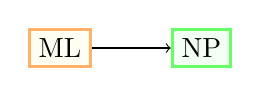
\begin{tikzpicture}[
roundnode/.style={rectangle, draw=green!60, fill=green!5, very thick, minimum size=4mm},
squarednode/.style={rectangle, draw=orange!60, fill=yellow!5, very thick, minimum size=4mm},
]
%Nodes
\node[squarednode]      (ml)                              {$\text{ML}$};
\node[roundnode]        (np)       		[right=of ml] {$\text{NP}$};

%Lines
\draw[->] (ml.east) -- (np.west);
\end{tikzpicture}
\end{center}

We begin with the well-known fundamental (non-unique) conversion of an ML problem into an NP problem.

An ML problem is about finding a function $f$ $\mathcal{X}\to \mathcal{Y}$ such that $\mathscr{L}(f):=\mathbb{E}_{(X,Y)\sim \mathcal{P}}l(f(X), Y)$ is small enough where $\mathcal{P}$ is an unknown distribution over $\mathcal{X}\times Y$ and $l:\mathcal{Y}\times \mathcal{Y} \to \mathbb{R}$ is a loss function, and we are given sampling from the unknown distribution $\mathcal{P}$ in a certain fashion (online or offline).

A model is a class $\mathcal{H}$ of functions from $\mathcal{X}$ to $\mathcal{Y}$ (called Hypothesis Space). We say the model is good if one of $f\in \mathcal{H}$ will make $\mathscr{L}(f)$ small enough.

Suppose that we're given enough data (the amount is still polynomial, which is possible if $\log \mathcal{H}$ is polynomial, which will be true if elements in $\mathcal{H}$ arer polynomially presentable), then $\widehat{\mathscr{L}}(f):=todo$ becomes a good approximation of $\mathscr{L}(f)$. Then whether the model is a good one becomes an NP problem, with the proof being the specific $f\in \mathcal{H}$ making $\widehat{\mathscr{L}}(f)$ small enough.

More generally, we could think of meta learning. Suppose we have a family of machine learning problems indexed by S, todo
\subsection{ML Problems Arising from NP Problems}
\begin{center}
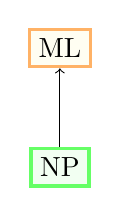
\begin{tikzpicture}[
roundnode/.style={rectangle, draw=green!60, fill=green!5, very thick, minimum size=4mm},
squarednode/.style={rectangle, draw=orange!60, fill=yellow!5, very thick, minimum size=4mm},
]
%Nodes
\node[roundnode]        (np)       		              {$\text{NP}$};
\node[squarednode]      (ml)           [above=of np]  {$\text{ML}$};

%Lines
\draw[->] (np.north) -- (ml.south);
\end{tikzpicture}
\end{center}

Given an NP problem, which consists of an input space $\mathcal{X}$, a certificate space $\mathcal{C}$, and a polytime verifier $v: \mathcal{X} \rightarrow \text{Bool}$, the goal is then to find an efficient implementation or approximation of $x\mapsto \exists_{c\in \mathcal{C}} v(x,c)$.

Let's start with some brute force method for find certificates, denoted by $c_{\text{brute}}(x): \mathcal{X} \to \mathcal{C}$.

Suppose that we are satisfied with the approximation $x\mapsto v(x,c_{\text{brute}}(x))$ and we only want to make it faster. We can collect a set of $x_i\in \mathcal{X}$, then build a dataset with $y_i=c_{brute}(x)$, then this becomes a machine learning problem.

(A more appropriate setup would be to make $c_{brute}(x)$ being a small finite set of certificates, and $v(x,c_{\text{brute}}(x))$ will become $\exists c\in c_{\text{brute}}(x), v(x, c)$)

Now in general we can't be satisfied with the simple approximation $x\mapsto v(x,c_{\text{brute}}(x))$, we can also use machine learning to make a better approximation.

One way is to divide and conquer. Factor $\mathcal{C}$ into a disjoint union $\sqcup_{i\in \mathcal{I}} \mathcal{C}_{i}$ indexed by a not necessarily small set $\mathcal{I}$. Then
\begin{equation}
	f_*(x)=\exists i\in \mathcal{I}, \exists c\in \mathcal{C}_i, v(x,c).
\end{equation}

Suppose that we have a brute force method $c_{\text{brute},i}$ for each $\mathcal{C}_i$. Define
\begin{equation}
	g: \mathcal{X}\times \mathcal{I} \rightarrow \text{Bool}, g(x, i) = v(x, c_{\text{brute},i}(x))
\end{equation}

Now $g$ is a function we can approximate with machine learning. Let the approximation we get be $\hat{g}$, then we can simplify the problem by searching within $\mathcal{I}$ of $s$

... RL is a special case.

\subsection{the Ladder of NP-ML Ascension}
``Good mathematicians see analogies. Great mathematicians see analogies between analogies.''

\hfill -- Stefan Banach, as in Banach Space


\begin{center}
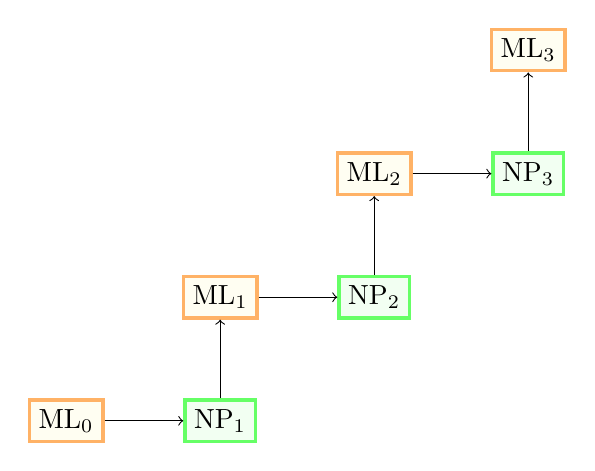
\begin{tikzpicture}[
roundnode/.style={rectangle, draw=green!60, fill=green!5, very thick, minimum size=4mm},
squarednode/.style={rectangle, draw=orange!60, fill=yellow!5, very thick, minimum size=4mm},
]
%Nodes
\node[squarednode]      (ml0)                              {$\text{ML}_0$};
\node[roundnode]        (np1)       		[right=of ml0] {$\text{NP}_1$};
\node[squarednode]      (ml1)       		[above=of np1] {$\text{ML}_1$};
\node[roundnode]        (np2)       		[right=of ml1] {$\text{NP}_2$};
\node[squarednode]      (ml2)       		[above=of np2] {$\text{ML}_2$};
\node[roundnode]        (np3)       		[right=of ml2] {$\text{NP}_3$};
\node[squarednode]      (ml3)       		[above=of np3] {$\text{ML}_3$};

%Lines
\draw[->] (ml0.east) -- (np1.west);
\draw[->] (np1.north) -- (ml1.south);
\draw[->] (ml1.east) -- (np2.west);
\draw[->] (np2.north) -- (ml2.south);
\draw[->] (ml2.east) -- (np3.west);
\draw[->] (np3.north) -- (ml3.south);
\end{tikzpicture}
\end{center}

The typical machine learnings algorithms including deep learning, typically doesn't go up beyond $NP_1$, that's why they can't achieve AGI and needs a lot of amount of data to fake AGI in restricted scenarios.

Todo: give many concrete examples. Many will come from programming and mathematics.

Todo: explain why it doesn't take much data to ascend.

\subsection{$NP_0$ Preceding $ML_0$: CV and NLP}


\section{AGI Theories Based on Realistic Computation Models}

\subsection{Locally Sensitive Hashing}



\section{Type System}

\subsection{Concept Level Types}


\subsection{System Level Types}

\subsection{Types for Machine Learning}

\section{Husky Programming Language}

Here we give a brief description of the Husky programming language, invented to implement the above ideas.

\subsection{Requirements for AGI-Ready Programming Language}

\subsection{}

\subsection{}

Here we lay down the requirements for a programming language that can implement the efficient AGI as we described.

\paragraph{Basic Requirements} We first discuss basic requirements, each of which is satisfied by at least one current programming language or is among the future design goals. However, there is no single language that satisfies all of them, a direct consequence of the fact that computer science has only been developed for 70 years.

\begin{enumerate}[(i)]
	\item purity.


We don't want to use a programming language with which we can shoot ourselves in the feet.

Logic errors is fine, but it can be detected in the debugger and handled in a controlled manner, but memory bugs and other undefined behaviors will make a large system extremely hard to track. One needs to know much more to debug a memory bug, than a logic one.

	\item modularity
	\item term level coding
	\item system level coding
	\item all level debugging support
	\item 
\end{enumerate}

\paragraph{Advanced Requirements}

\begin{enumerate} [(i)]
	\item express evolving computation graph
\end{enumerate}

\section{Plans for Computer Vision}

\section{Plans for Natural Language Processing}

As claimed in previous sections, deep learning's success doesn't mean it's the optimal for natural language processing, but it will serve as a convenient tool for the development of a next generation far more superior tools.

Let's first conduct a worst scenario analysis. Suppose deep learning achieved AGI before us, and the AGI works amazingly well. Let's recall what makes symbolic AI methods like expert system fail: high development, maintenance, and debugging cost. But we can instruct deep learning AGI develop expert system and write out programs that parse English like parsing a programming language. It would take forever for humans, but for AGI, it would be trivial. The takeaway is, even if deep learning takes the holy grail, it won't keep it for very long as humans could then replace it a more rule-based AI with its help.

But this argument is not satisfying, due to the gloomy prospect of deep learning achieving AGI. Still there could be many practical approaches where we can leverage deep learning in its current form to build a more advanced form of AI, which I shall explain below.

\subsection{Stage 0: Domain Specific Verifiable Natural Language Processing}

We shall restrict ourselves to a very specific domain, relatively simple, so that we can easily build up a domain specific programming langauge to describe the tasks and also build efficient solvers for the task.
\begin{center}
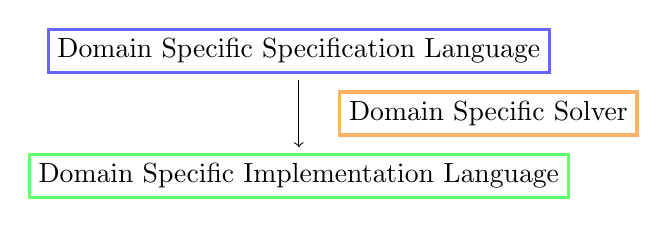
\begin{tikzpicture}[
squarednode1/.style={rectangle, draw=blue!60, fill=white!5, very thick, minimum size=4mm},
squarednode2/.style={rectangle, draw=green!60, fill=white!5, very thick, minimum size=4mm},
squarednode3/.style={rectangle, draw=orange!60, fill=white!5, very thick, minimum size=4mm},
]
%Nodes
\node[squarednode1]      (dssl)                              {Domain Specific Specification Language};
\node[squarednode2]      (dsil)              [below=of dssl]  {Domain Specific Implementation Language};

%Lines
\draw[->, shorten >=2pt, shorten <=2pt] (dssl.south) -- (dsil.north) node[squarednode3, midway, right, xshift=5mm] {Domain Specific Solver};
\end{tikzpicture}
\end{center}

\begin{eg}
	[Mathematica]
\end{eg}

\begin{eg}
	[Html, Css] Html and Css are not specification languages, they are implementation languages.
\end{eg}

Let's compare the pros and cons with ChatGPT

Here's a nice summary in table \ref{comparison} written by the very ChatGPT itself.

\begin{table}[ht]
\label{comparison}
\centering
\small % reduce font size
\begin{tabular}{|l|p{6cm}|p{6cm}|}
\hline
 & \textbf{ChatGPT} & \textbf{DSLs} \\
\hline
\textbf{Pros} & 
Flexibility: ChatGPT can be used for a wide variety of NLP tasks, including text generation, question answering, summarization, and more.
&
Increased productivity: DSLs are designed to be easy to use and understand within a specific domain, which can increase developer productivity. \\
\cline{2-3}
& 
Ease of use: ChatGPT can be accessed through simple API calls or integrated into other applications and platforms.
&
Enhanced control: A DSL provides more fine-grained control over a specific problem within a domain, allowing developers to tailor their solutions to specific requirements. \\
\cline{2-3}
& 
Low development time: Implementing a ChatGPT-based solution typically requires less development time than creating a custom DSL.
&
Improved maintainability: DSLs can make code more readable and maintainable within a specific domain, as they typically use domain-specific terminology and concepts. \\
\cline{2-3}
& 
Multilingual support: ChatGPT can generate text in multiple languages.
&
 \\
\hline
\textbf{Cons} & 
Limited control: ChatGPT generates text based on its training data and can sometimes produce unexpected or incorrect output.
&
Higher development time: Developing a custom DSL can require a significant amount of time and effort. \\
\cline{2-3}
& 
Lack of transparency: It can be difficult to understand why ChatGPT generates a particular piece of text, making it hard to debug or fine-tune.
&
Limited flexibility: A DSL is designed to solve a specific problem within a specific domain, so it may not be suitable for other tasks or domains. \\
\cline{2-3}
& 
Dependence on data quality: The quality of ChatGPT's output is heavily dependent on the quality and diversity of its training data.
&
Steep learning curve: Developers may need to learn a new syntax and programming paradigm in order to use a DSL effectively. \\
\hline
\end{tabular}
\caption{Comparison of ChatGPT and DSLs}
\label{tab:chatgpt-dsls}
\end{table}

I'm sorry that I have to copy because my hands are not in 100\% health.

\clearpage

We could have the best of both worlds by combining dsls with deep learning like this:
\begin{center}
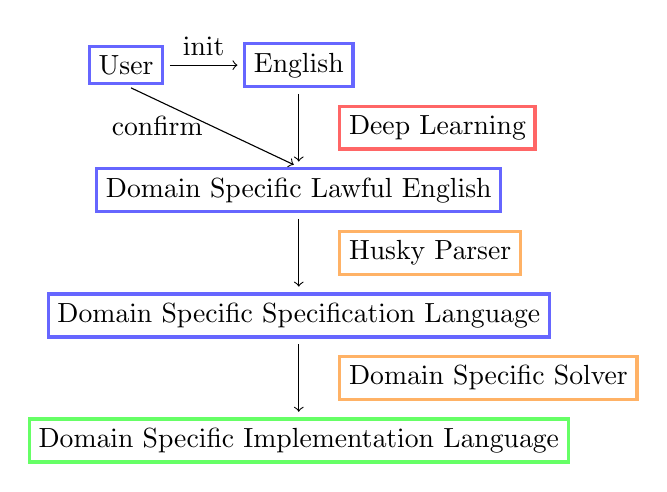
\begin{tikzpicture}[
squarednode1/.style={rectangle, draw=blue!60, fill=white!5, very thick, minimum size=4mm},
squarednode2/.style={rectangle, draw=green!60, fill=white!5, very thick, minimum size=4mm},
squarednode3/.style={rectangle, draw=orange!60, fill=white!5, very thick, minimum size=4mm},
squarednode4/.style={rectangle, draw=red!60, fill=white!5, very thick, minimum size=4mm},
]
%Nodes
\node[squarednode1]              (user)                              {User};
\node[squarednode1]      (e)             [right=of user]   {English};
\node[squarednode1]      (dsle)             [below=of e]   {Domain Specific Lawful English};
\node[squarednode1]      (dssl)             [below=of dsle]    {Domain Specific Specification Language};
\node[squarednode2]      (dsil)              [below=of dssl]  {Domain Specific Implementation Language};

%Lines
\draw[->, shorten >=2pt, shorten <=2pt] (user.east) -- (e.west) node[midway, above] {init};
\draw[->, shorten >=2pt, shorten <=2pt] (user.south) -- (dsle.north) node[midway, left] {confirm};
\draw[->, shorten >=2pt, shorten <=2pt] (e.south) -- (dsle.north) node[squarednode4, midway, right, xshift=5mm] {Deep Learning};
\draw[->, shorten >=2pt, shorten <=2pt] (dsle.south) -- (dssl.north) node[squarednode3, midway, right, xshift=5mm] {Husky Parser};
\draw[->, shorten >=2pt, shorten <=2pt] (dssl.south) -- (dsil.north) node[squarednode3, midway, right, xshift=5mm] {Domain Specific Solver};
\end{tikzpicture}
\end{center}

First, we create a subset of English called Domain Specific Lawful English such as
\begin{enumerate}[(i)]
	\item it's grammarly and semantically rigorous, so that parsing in Husky code is feasible (although it might be too difficult for traditional languages like C++/Rust/Python/Haskell)
	\item it's expressive enough for the domain and can be faithfully translated into the Domain Specific Specification Language
	\item easily understood by users
\end{enumerate}

Second, we collect data and train a deep neural network that can translate arbitrary English into the subset.

When user initializes a dialogue using arbitrary English, it's translated into Domain Specific Lawful English, which is checked by the Husky Parser and also confirmed by the user that the translation is correct.

Then the Domain Specific Lawful English is translated by the Husky Parser into Domain Specific Specification Language so that it's acceptable by the solver.

Obviously, this setup will have the advantages of both worlds.

The details will be covered in the followup papers.

\subsection{Stage 1: Universal Lawful English}

Todo

\subsection{Stage 2: Minimizing Usage of Deep Learning}

Todo

\subsection{Stage 3: Learning Augmented Verifiable Solver}

Todo

\subsection{Stage 4: Generating Human Readable Explanations}

Todo

\end{document}